% =============================================================================
% Relatório - Trabalho de Implementação de Rede Neural MLP
% Compilar com:  cd relatorio && tectonic relatorio.tex
% =============================================================================
\documentclass[11pt,a4paper]{article}
\usepackage[utf8]{inputenc}
\usepackage[T1]{fontenc}
\usepackage[brazil]{babel}
\usepackage{lmodern}
\usepackage[margin=2.4cm]{geometry}
\usepackage{graphicx}
\usepackage{booktabs}
\usepackage{amsmath,amssymb}
\usepackage{xcolor}
\usepackage{float}
\usepackage{caption}
\usepackage{enumitem}
\usepackage{listings}
\usepackage{xurl}
\usepackage[hidelinks]{hyperref}
\urlstyle{same}

\graphicspath{{../figuras/}}
\captionsetup{font=small,labelfont=bf}
\setlist{nosep}
\lstset{basicstyle=\ttfamily\footnotesize,breaklines=true,frame=single,framerule=0.3pt,
  rulecolor=\color{gray!60},columns=fullflexible,keepspaces=true,
  literate={á}{{\'a}}1 {à}{{\`a}}1 {ã}{{\~a}}1 {â}{{\^a}}1 {é}{{\'e}}1 {ê}{{\^e}}1 {í}{{\'i}}1
           {ó}{{\'o}}1 {õ}{{\~o}}1 {ô}{{\^o}}1 {ú}{{\'u}}1 {ç}{{\c{c}}}1 {É}{{\'E}}1}

\newcommand{\alunos}{Pedro Henrique Porto França Cornutti\\Ramon Mielke}
\newcommand{\semestre}{2026/4}

\title{\textbf{Previsão de Desempenho de Jogadores de Basquete\\com uma Rede Neural MLP Implementada do Zero}}
\author{\alunos\\[4pt]\small FBX4054 -- Inteligência Computacional\\\small Universidade de Caxias do Sul}
\date{\small Semestre \semestre}

\begin{document}
\maketitle

\begin{abstract}
Este trabalho implementa, em Python puro (sem bibliotecas de aprendizado de máquina), uma rede neural
perceptron multicamadas (MLP) para classificar jogadores da NBA em desempenho \emph{Good} ou \emph{Bad}
a partir de 31 atributos estatísticos da temporada. O relatório cobre os cinco itens do projeto:
preparação dos dados, implementação do modelo, treinamento, avaliação/ajuste e interpretação.
A configuração final (31--16--1, ativação sigmoide, taxa de aprendizado 0,1, 110 épocas), escolhida
por validação cruzada estratificada de 5 \emph{folds}, obteve no conjunto de teste (153 jogadores) acurácia
média de 0,974, recall de 0,947, precisão de 0,818, F1 de 0,877 e AUC de 0,995 em cinco execuções
independentes. A análise de importância mostra que o rótulo é quase inteiramente explicado pelos pontos
por jogo (PTS) e seus componentes; sem os atributos de pontuação, a rede ainda atinge AUC de 0,981,
apoiando-se principalmente em erros de posse (TOV) e minutos por jogo (MP).
\end{abstract}

\tableofcontents
\vspace{1em}

% =============================================================================
\section{Introdução}
O objetivo do trabalho é construir uma rede neural MLP do zero e usá-la para prever o desempenho de
jogadores de basquete, conforme o enunciado da Atividade Avaliativa 2 da disciplina (BOFF, 2026). O dataset,
disponibilizado no ambiente virtual junto com o enunciado, contém estatísticas por jogo de jogadores da NBA
(os registros indicam a temporada 2022--23, até aproximadamente fevereiro de 2023) e um atributo alvo
\texttt{Performance} com dois valores: \emph{Good} (52 instâncias) e \emph{Bad} (570 instâncias).

A MLP é o modelo conexionista clássico para aprendizado supervisionado: neurônios artificiais organizados em
camadas, treinados pelo algoritmo de retropropagação do erro (HAYKIN, 2001; SILVA et al., 2018;
FACELI et al., 2021; RUSSELL; NORVIG, 2022). Ela generaliza o perceptron de Rosenblatt (1958), que só separa classes linearmente,
e se tornou prática com a formulação do \emph{backpropagation} por Rumelhart, Hinton e Williams (1986).

\subsection*{Relação com o plano de ensino}
O trabalho aplica dois itens do conteúdo programático da disciplina FBX4054. O item 4, \emph{Sistemas
Conexionistas} (fundamentos e principais modelos de redes neurais), é a base da implementação da
Seção~\ref{sec:modelo}, que segue os slides de redes neurais artificiais da Aula 9 (ADAMI; BOFF, 2026) e a
bibliografia básica (FACELI et al., 2021; LUGER, 2013; RUSSELL; NORVIG, 2022). O item 3, \emph{Aprendizagem
Automática} (paradigmas de aprendizagem), fundamenta o tratamento do problema como classificação
supervisionada e o protocolo de avaliação das Seções~\ref{sec:treino} e~\ref{sec:avaliacao}, que segue os
slides de métodos de avaliação de desempenho da Aula 7 (ADAMI, 2026). O trabalho exercita as competências
C1 (resolver problemas modelando soluções com metodologias de IA) e C2 (modelar sistemas inteligentes com
aquisição automática de conhecimento), em especial a habilidade de implementar a representação de
conhecimento em um sistema computacional (C1-H2) e de analisar metodologias de extração de conhecimento
para um problema indicado (C2-H2).

Todo o código foi escrito em Python 3.14. Seguindo o enunciado, a única biblioteca externa usada na
preparação dos dados foi o \texttt{pandas} (MCKINNEY, 2010); a rede neural, o treinamento e todas as métricas foram
implementados apenas com listas, \texttt{math} e \texttt{random}. O \texttt{matplotlib} (HUNTER, 2007) foi
utilizado exclusivamente para desenhar as figuras do relatório. O código completo acompanha a entrega
(Apêndice~\ref{apx:codigo}).

O relatório segue os cinco itens do projeto: Seção~\ref{sec:dados} (preparação dos dados),
Seção~\ref{sec:modelo} (implementação), Seção~\ref{sec:treino} (treinamento e ajuste de
hiperparâmetros), Seção~\ref{sec:avaliacao} (avaliação no conjunto de teste) e
Seção~\ref{sec:interpretacao} (interpretação e conclusão).

% =============================================================================
\section{Preparação dos dados}\label{sec:dados}

\subsection{Carga e inspeção}
O arquivo CSV foi carregado com \texttt{pandas} e inspecionado (dimensões, primeiras linhas, tipos e
valores faltantes). O dataset bruto possui 624 linhas e 31 colunas: 4 de identificação
(\texttt{Player}, \texttt{Tm}, \texttt{Pos}, \texttt{Age}), 26 estatísticas numéricas e o alvo.
A inspeção revelou quatro problemas, resumidos na Tabela~\ref{tab:prep}:

\begin{enumerate}
  \item \textbf{Coluna duplicada.} A coluna \texttt{FG\%.1} repete \texttt{FG\%} como texto com vírgula
        decimal (\texttt{"0,482"}). Foi descartada.
  \item \textbf{Linhas sem rótulo.} Duas linhas não têm \texttt{Performance} (uma delas é totalmente vazia).
        Como não servem para treinar nem avaliar um classificador supervisionado, foram removidas.
  \item \textbf{Jogadores repetidos.} 57 jogadores que trocaram de time durante a temporada aparecem em
        múltiplas linhas: uma com \texttt{Tm = TOT} (total da temporada) e uma por time. Manter todas
        colocaria o mesmo jogador, com estatísticas quase idênticas, em treino e teste ao mesmo tempo,
        o que inflaria artificialmente as métricas (\emph{vazamento}). Mantivemos apenas a linha TOT de cada
        um, removendo 114 linhas.
  \item \textbf{Valores faltantes.} Os percentuais de arremesso ficam vazios quando o jogador não tentou
        nenhum arremesso daquele tipo (divisão $0/0$). Verificamos no código que todo percentual faltante
        corresponde a zero tentativas e preenchemos com 0, que é o valor que o próprio dataset usa em
        casos equivalentes (Tabela~\ref{tab:faltantes}).
\end{enumerate}

\begin{table}[H]\centering\small
\begin{tabular}{lr}
\toprule
Etapa & Linhas \\
\midrule
Dataset bruto & 624 \\
Linhas sem rótulo removidas & $-$2 \\
Linhas por time de 57 jogadores trocados (mantida a linha TOT) & $-$114 \\
\textbf{Dataset limpo} & \textbf{508} \\
\quad classe Good & 49 \\
\quad classe Bad & 459 \\
\midrule
Treino (70\%) & 355 (34 Good) \\
Teste (30\%) & 153 (15 Good) \\
\bottomrule
\end{tabular}

\caption{Efeito de cada etapa da limpeza e divisão treino/teste.}\label{tab:prep}
\end{table}

\begin{table}[H]\centering\small
\begin{tabular}{lrl}
\toprule
Coluna & Faltantes & Causa / tratamento \\
\midrule
FG\% & 2 & FGA = 0 (divisão 0/0); preenchido com 0 \\
3P\% & 19 & 3PA = 0 (divisão 0/0); preenchido com 0 \\
2P\% & 5 & 2PA = 0 (divisão 0/0); preenchido com 0 \\
FT\% & 33 & FTA = 0 (divisão 0/0); preenchido com 0 \\
eFG\% & 2 & FGA = 0 (divisão 0/0); preenchido com 0 \\
\bottomrule
\end{tabular}

\caption{Valores faltantes após a remoção das linhas sem rótulo e das linhas por time.}\label{tab:faltantes}
\end{table}

\subsection{Codificação dos atributos}
A posição (\texttt{Pos}) é categórica com cinco valores (PG, SG, SF, PF, C); quatro jogadores tinham
posição dupla (ex.: \texttt{PF-SF}) e ficaram com a primeira. A posição foi codificada em cinco variáveis
binárias (\emph{one-hot}). O nome do jogador é um identificador e o time tem 30 valores com pouca
relação com o desempenho individual; ambos foram descartados. O alvo foi mapeado para
$y = 1$ (\emph{Good}) e $y = 0$ (\emph{Bad}). Resultam \textbf{31 atributos de entrada}: Age, G, GS, MP, FG, FGA, FG\%, 3P, 3PA, 3P\%, 2P, 2PA, 2P\%,
eFG\%, FT, FTA, FT\%, ORB, DRB, TRB, AST, STL, BLK, TOV, PF, PTS e as cinco variáveis de posição
(Pos\_PG, Pos\_SG, Pos\_SF, Pos\_PF, Pos\_C).

\subsection{Divisão treino/teste}
O dataset limpo (508 jogadores, 49 \emph{Good}) foi dividido em 70\% para treino e 30\% para teste de forma
\textbf{estratificada} (a mesma proporção de classes nos dois conjuntos), o \emph{stratified hold out}
apresentado por Adami (2026), com semente fixa (42) para reprodutibilidade. A divisão foi implementada manualmente: os índices de cada classe são embaralhados e
30\% deles vão para o teste. Resultado: 355 jogadores no treino (34 \emph{Good}) e 153 no teste (15 \emph{Good}),
Figura~\ref{fig:classes}. O conjunto de teste foi reservado e usado \textbf{uma única vez}, na avaliação final
(Seção~\ref{sec:avaliacao}); toda a escolha de hiperparâmetros usou apenas o treino.

\begin{figure}[H]\centering
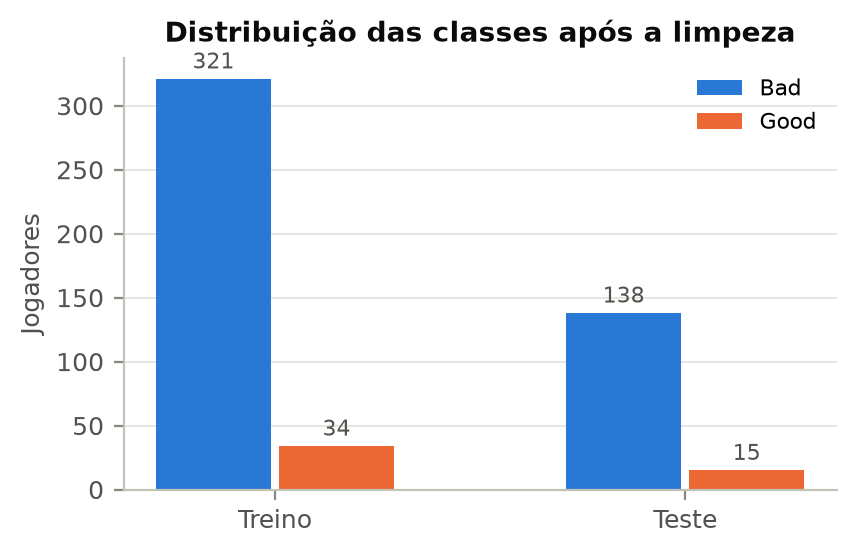
\includegraphics[width=0.55\textwidth]{fig01_classes.png}
\caption{Distribuição das classes nos conjuntos de treino e teste. O desbalanceamento é forte: apenas 9,6\% das instâncias são \emph{Good}.}\label{fig:classes}
\end{figure}

\subsection{Padronização}
As 26 variáveis numéricas têm escalas muito diferentes (idade em anos, minutos, pontos, percentuais
entre 0 e 1). Como a MLP usa ativação sigmoide e descida do gradiente, entradas em escalas distintas
fariam alguns pesos dominarem o gradiente e dificultariam a convergência. Entre as heurísticas de treino
da MLP, Haykin (2001) e Adami e Boff (2026) recomendam normalizar as entradas para média próxima de zero,
o que acelera a convergência. Cada variável foi, então, padronizada (\emph{z-score}):
\[
  x' = \frac{x - \mu_{\text{treino}}}{\sigma_{\text{treino}}},
\]
com média e desvio padrão calculados \textbf{apenas no conjunto de treino} e depois aplicados ao teste,
evitando que informação do teste influencie o pré-processamento. As cinco variáveis binárias de posição
não foram padronizadas. As médias e desvios usados ficam salvos no arquivo \texttt{padronizacao.json},
na pasta \texttt{dados/processados}.

\subsection{Análise exploratória}
A Tabela~\ref{tab:estat} apresenta a média de cada atributo por classe e a correlação de Pearson com o
alvo (equivalente à correlação ponto-bisserial, pois o alvo é binário); a Figura~\ref{fig:corr} ordena
os atributos por essa correlação. Os atributos mais associados ao rótulo \emph{Good} são todos de
\textbf{volume de pontuação}: lances livres convertidos (FT, $r=0{,}74$), pontos por jogo (PTS, 0,74),
lances livres tentados (FTA, 0,72), cestas de quadra (FG, 0,71) e tentativas (FGA, 0,70). Em seguida vêm
erros de posse (TOV, 0,65), assistências (AST, 0,55) e minutos (MP, 0,49). Os percentuais de aproveitamento
(FG\%, 2P\%, eFG\%) quase não se correlacionam com o alvo: ser \emph{Good} não é ser eficiente, é
\emph{produzir volume}.

A Figura~\ref{fig:pts} torna isso explícito: todos os 49 jogadores \emph{Good} têm pelo menos 20,5 pontos por
jogo e apenas um jogador \emph{Bad} (Terry Rozier, 21,4 PTS) ultrapassa 20 pontos. Ou seja, o rótulo é,
na prática, ``jogador que marca 20 ou mais pontos por jogo''. Essa observação orienta a interpretação dos
resultados na Seção~\ref{sec:interpretacao}.

\begin{figure}[H]\centering
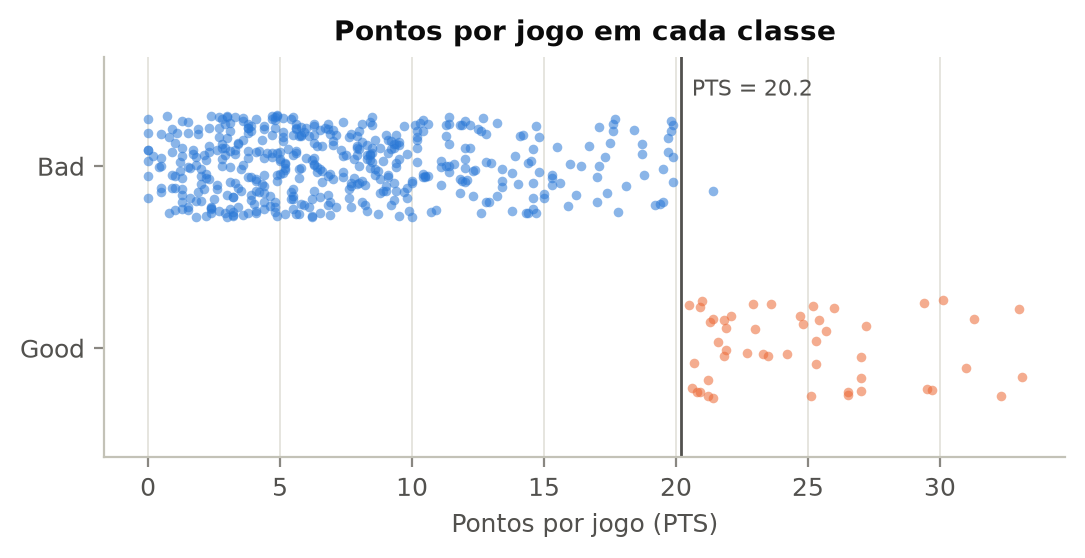
\includegraphics[width=0.85\textwidth]{fig02_pts_por_classe.png}
\caption{Pontos por jogo (PTS) de cada jogador, separados por classe. A linha vertical marca o limiar de
20,2 PTS escolhido no conjunto de treino para a regra de referência da Seção~\ref{sec:baselines}.}\label{fig:pts}
\end{figure}

\begin{figure}[H]\centering
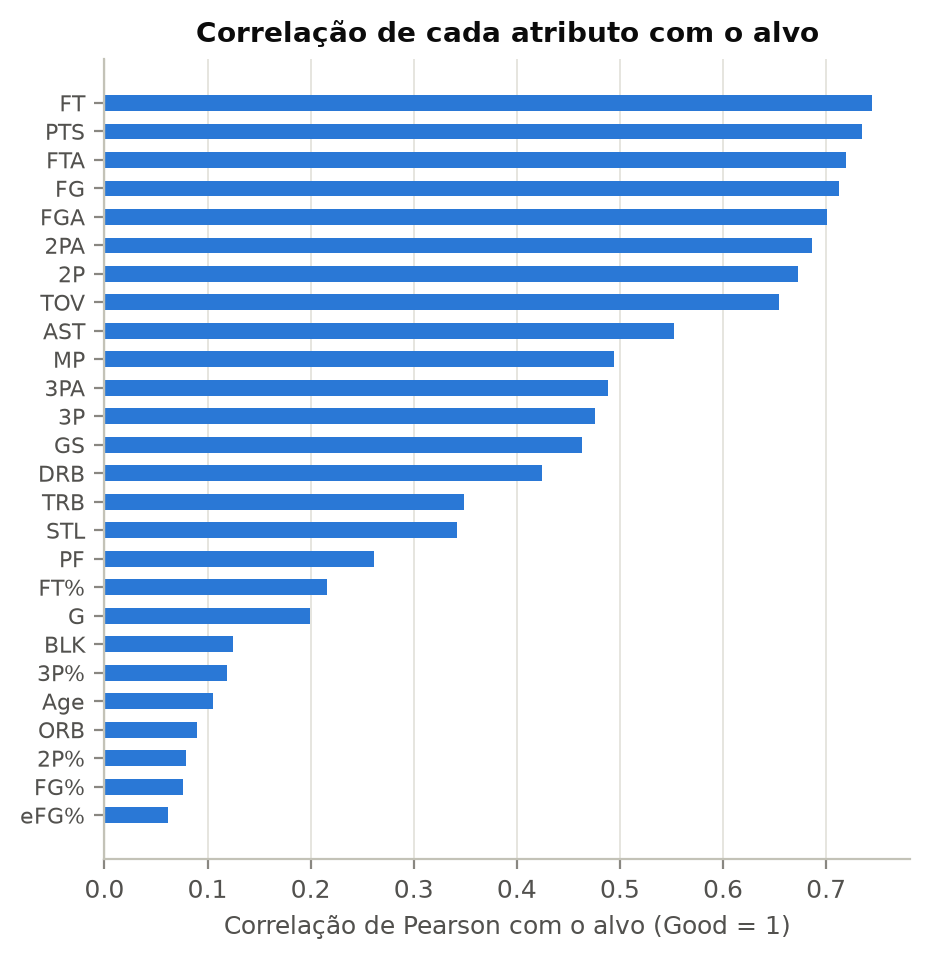
\includegraphics[width=0.62\textwidth]{fig03_correlacao_alvo.png}
\caption{Correlação de Pearson de cada atributo numérico com o alvo (\emph{Good} = 1), no dataset limpo.}\label{fig:corr}
\end{figure}

\begin{table}[H]\centering\small
\begin{tabular}{lrrrr}
\toprule
Atributo & Média Bad & Média Good & Desvio padrão & Correlação com o alvo \\
\midrule
FT & 1,059 & 5,041 & 1,579 & 0,745 \\
PTS & 7,351 & 24,782 & 7,000 & 0,735 \\
FTA & 1,410 & 6,098 & 1,924 & 0,719 \\
FG & 2,732 & 8,731 & 2,487 & 0,712 \\
FGA & 5,864 & 18,053 & 5,134 & 0,701 \\
2PA & 3,496 & 11,873 & 3,602 & 0,687 \\
2P & 1,896 & 6,473 & 2,009 & 0,673 \\
TOV & 0,919 & 2,804 & 0,850 & 0,654 \\
AST & 1,661 & 5,251 & 1,917 & 0,553 \\
MP & 18,050 & 34,604 & 9,887 & 0,494 \\
3PA & 2,369 & 6,180 & 2,303 & 0,488 \\
3P & 0,836 & 2,261 & 0,885 & 0,476 \\
GS & 14,778 & 48,490 & 21,481 & 0,463 \\
DRB & 2,398 & 5,047 & 1,841 & 0,425 \\
TRB & 3,237 & 6,100 & 2,427 & 0,348 \\
STL & 0,564 & 1,020 & 0,394 & 0,342 \\
PF & 1,633 & 2,353 & 0,812 & 0,262 \\
FT\% & 0,643 & 0,835 & 0,262 & 0,216 \\
G & 36,978 & 49,041 & 17,853 & 0,199 \\
BLK & 0,364 & 0,529 & 0,391 & 0,124 \\
3P\% & 0,298 & 0,355 & 0,140 & 0,119 \\
Age & 25,645 & 27,204 & 4,366 & 0,105 \\
ORB & 0,842 & 1,069 & 0,751 & 0,089 \\
2P\% & 0,500 & 0,542 & 0,155 & 0,079 \\
FG\% & 0,453 & 0,484 & 0,120 & 0,077 \\
eFG\% & 0,521 & 0,547 & 0,123 & 0,062 \\
\bottomrule
\end{tabular}

\caption{Estatísticas descritivas por classe (valores originais, antes da padronização) e correlação com o alvo.}\label{tab:estat}
\end{table}

% =============================================================================
\section{Implementação do modelo}\label{sec:modelo}

A rede está em \texttt{src/mlp.py} (classe \texttt{MLP}) e foi escrita apenas com listas Python e os módulos
\texttt{math} e \texttt{random}. Esta seção descreve cada componente.

\subsection{Arquitetura}
A MLP é totalmente conectada e \emph{feed-forward}, com camada de entrada, camadas ocultas e camada de
saída (HAYKIN, 2001; ADAMI; BOFF, 2026). A arquitetura é parametrizada pelo número de entradas,
por uma lista com o número de neurônios de cada camada oculta e pela função de ativação das camadas ocultas.
A camada de saída tem sempre um neurônio com ativação sigmoide, que produz $\hat y \in (0,1)$, interpretado
como a probabilidade estimada de a instância ser \emph{Good}; a classe prevista é \emph{Good} quando
$\hat y \ge 0{,}5$. A configuração final, escolhida na Seção~\ref{sec:treino}, é \textbf{31--16--1}
(Figura~\ref{fig:arq}): 31 entradas, uma camada oculta com 16 neurônios sigmoides e um neurônio de saída,
totalizando $31\cdot16 + 16 + 16\cdot1 + 1 = 529$ parâmetros treináveis.

\begin{figure}[H]\centering
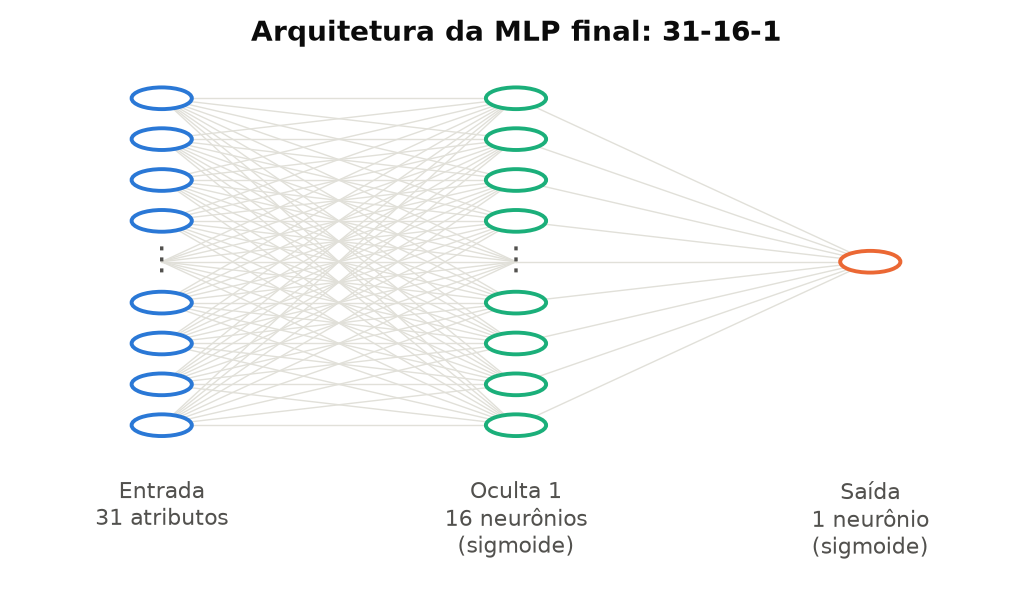
\includegraphics[width=0.8\textwidth]{fig04_arquitetura.png}
\caption{Arquitetura da MLP final. Apenas parte dos nós de cada camada é desenhada.}\label{fig:arq}
\end{figure}

\subsection{Inicialização dos pesos}
Os pesos são armazenados como \texttt{pesos[l][j][i]} (peso da entrada $i$ para o neurônio $j$ da camada $l$)
e os vieses como \texttt{vieses[l][j]}. Os vieses iniciam em zero. Os pesos são sorteados de uma distribuição
uniforme, como sugerem as heurísticas de Adami e Boff (2026), com a inicialização de \textbf{Glorot}
(GLOROT; BENGIO, 2010) para sigmoide/tanh e de \textbf{He} (HE et al., 2015) para ReLU:
\[
  w_{\text{Glorot}} \sim \mathcal{U}\!\left(\pm\sqrt{\frac{6}{n_{\text{in}}+n_{\text{out}}}}\right),
  \qquad
  w_{\text{He}} \sim \mathcal{U}\!\left(\pm\sqrt{\frac{6}{n_{\text{in}}}}\right).
\]
Essas escalas mantêm a variância das ativações estável entre camadas e evitam que a sigmoide sature logo
no início do treino. A semente do gerador é um parâmetro, o que permite repetir execuções e também variar a
inicialização entre execuções (Seção~\ref{sec:execucoes}).

\subsection{Funções de ativação}
Foram implementadas três ativações para as camadas ocultas, com as derivadas escritas em função da própria
ativação $a = f(z)$, o que evita recomputar $z$ na retropropagação:
\[
\begin{array}{lll}
\text{sigmoide:} & \sigma(z) = \dfrac{1}{1+e^{-z}}, & \sigma'(z) = a(1-a);\\[8pt]
\text{tanh:} & \tanh(z) = \dfrac{e^{z}-e^{-z}}{e^{z}+e^{-z}}, & \tanh'(z) = 1-a^2;\\[8pt]
\text{ReLU:} & \max(0, z), & f'(z) = [a>0].
\end{array}
\]
A sigmoide foi implementada de forma numericamente estável (usando $e^{z}/(1+e^{z})$ quando $z<0$) para não
provocar \emph{overflow} em $e^{-z}$.

\subsection{Propagação direta}
Para uma entrada $\mathbf{a}^{(0)} = \mathbf{x}$, cada camada $l$ calcula
\[
  z^{(l)}_j = \sum_i w^{(l)}_{ji}\, a^{(l-1)}_i + b^{(l)}_j, \qquad a^{(l)}_j = f\!\left(z^{(l)}_j\right),
\]
com $f$ = ativação escolhida nas camadas ocultas e $f = \sigma$ na saída. O método \texttt{propagar}
devolve a lista de ativações de todas as camadas, pois elas são necessárias na retropropagação.

\subsection{Função de perda}
Como a tarefa é classificação binária com saída sigmoide, usamos a \textbf{entropia cruzada binária}
(GOODFELLOW; BENGIO; COURVILLE, 2016), com um
peso opcional $w_+$ para a classe positiva que permite compensar o desbalanceamento (9,4 jogadores \emph{Bad}
para cada \emph{Good} no treino):
\[
  L = -\frac{1}{N}\sum_{n=1}^{N}\Big[\, w_+\, y_n \log \hat y_n + (1-y_n)\log(1-\hat y_n) \Big].
\]
Com $w_+ = 1$ é a entropia cruzada padrão; com $w_+ = 9{,}4$ cada jogador \emph{Good} pesa tanto quanto
9,4 jogadores \emph{Bad}. O efeito de $w_+$ foi avaliado como hiperparâmetro (Seção~\ref{sec:grid}).

\subsection{Retropropagação}
O gradiente é obtido pelo algoritmo de retropropagação (RUMELHART; HINTON; WILLIAMS, 1986), que alterna
uma fase \emph{forward}, em que a rede produz a saída e o erro, e uma fase \emph{backward}, em que o erro é
propagado da saída para a entrada pela regra da cadeia (HAYKIN, 2001; ADAMI; BOFF, 2026). Para a combinação
sigmoide + entropia
cruzada o erro do neurônio de saída simplifica para
\[
  \delta^{(L)} = \frac{\partial L_n}{\partial z^{(L)}} = w_n\,(\hat y_n - y_n), \qquad
  w_n = \begin{cases} w_+ & y_n = 1\\ 1 & y_n = 0,\end{cases}
\]
e para cada camada oculta, de $l = L-1$ até 1,
\[
  \delta^{(l)}_i = f'\!\left(z^{(l)}_i\right)\sum_j w^{(l+1)}_{ji}\,\delta^{(l+1)}_j .
\]
Os gradientes dos parâmetros são
$\partial L_n/\partial w^{(l)}_{ji} = \delta^{(l)}_j\, a^{(l-1)}_i$ e
$\partial L_n/\partial b^{(l)}_j = \delta^{(l)}_j$. Na classe, o método \texttt{gradientes} chama
\texttt{\_retropropagar} para cada instância do lote, soma os gradientes em acumuladores e divide pelo
tamanho do lote. O trecho central é:

\begin{lstlisting}[language=Python]
delta = [peso * (ativacoes[-1][0] - y)]           # erro na saída
for l in range(len(self.pesos) - 1, -1, -1):
    a_ant = ativacoes[l]                            # ativações da camada anterior
    for j, dj in enumerate(delta):
        acum_b[l][j] += dj
        for i, ai in enumerate(a_ant):
            acum_W[l][j][i] += dj * ai
    if l > 0:                                       # propaga o erro para trás
        W = self.pesos[l]
        delta = [self.df(a_ant[i]) * sum(W[j][i] * delta[j] for j in range(len(delta)))
                 for i in range(len(a_ant))]
\end{lstlisting}

\subsection{Descida do gradiente}
O treinamento usa \textbf{descida do gradiente em mini-lotes}: a cada época, as instâncias de treino são
embaralhadas e divididas em lotes de 32; para cada lote calcula-se o gradiente médio e atualiza-se cada
parâmetro na direção oposta ao gradiente:
\[
  w \leftarrow w - \eta\left(\frac{1}{m}\sum_{n \in \text{lote}} \frac{\partial L_n}{\partial w} + \lambda w\right),
  \qquad b \leftarrow b - \eta\,\frac{1}{m}\sum_{n \in \text{lote}} \frac{\partial L_n}{\partial b},
\]
onde $\eta$ é a taxa de aprendizado e $\lambda$ um termo opcional de regularização L2 (mantido em zero nos
experimentos). Com lote igual ao tamanho do conjunto o método vira a descida do gradiente clássica
(\emph{batch}); o mini-lote foi preferido por convergir em menos épocas com o mesmo custo por época
(GOODFELLOW; BENGIO; COURVILLE, 2016).
Ao fim de cada época (ou a cada $k$ épocas) o método \texttt{treinar} registra a perda de treino e, se
houver um conjunto de validação, a perda, a acurácia e o F1 de validação, produzindo as curvas da
Seção~\ref{sec:epocas}.

\subsection{Verificação da implementação}
Antes dos experimentos, a corretude da rede foi verificada com 8 testes automatizados, todos aprovados,
no arquivo \texttt{tests/test\_mlp.py}:
\begin{itemize}
  \item \textbf{Checagem numérica do gradiente}: para uma rede 4--5--3--1 com cada uma das três ativações, o
        gradiente analítico da retropropagação foi comparado com diferenças finitas centrais
        ($\varepsilon = 10^{-6}$) em todos os 529 parâmetros; o maior erro relativo ficou abaixo de $10^{-5}$,
        inclusive com $w_+ = 5$. Isso confirma que a retropropagação está correta.
  \item \textbf{Aprendizado do XOR}: uma rede 2--8--1 com tanh aprende o problema XOR (não linearmente
        separável) com 100\% de acerto, mostrando que a camada oculta e o treinamento funcionam.
  \item \textbf{Métricas}: matriz de confusão, acurácia, precisão, recall, especificidade, F1 e AUC foram
        conferidos contra valores calculados à mão, incluindo os casos de divisão por zero e de empate de
        pontuações na curva ROC.
\end{itemize}

% =============================================================================
\section{Treinamento do modelo e ajuste de hiperparâmetros}\label{sec:treino}

\subsection{Protocolo}
Para escolher os hiperparâmetros sem tocar no conjunto de teste, usamos \textbf{validação cruzada
estratificada com 5 \emph{folds}} dentro do treino, seguindo a recomendação de Adami (2026) de selecionar
hiperparâmetros apenas nos dados de treinamento e a análise de Kohavi (1995), que favorece a validação
cruzada estratificada para estimar a acurácia e escolher modelos: os 355 jogadores são divididos em 5 partes com a mesma
proporção de classes ($\approx$ 71 jogadores e 7 \emph{Good} por parte); cada configuração é treinada 5 vezes,
cada vez validando na parte deixada de fora. A métrica principal de seleção foi o \textbf{F1 da classe
\emph{Good}} (média dos 5 \emph{folds}), com a AUC como desempate, porque com 90\% de instâncias \emph{Bad} a
acurácia sozinha é pouco informativa (um modelo que diz sempre \emph{Bad} acerta 90\%). Os 24 treinamentos
de cada rodada foram paralelizados em 8 processos; o grid completo (120 treinamentos de 300 épocas) levou
239 s.

\subsection{Grid de hiperparâmetros}\label{sec:grid}
A primeira rodada combinou, com ativação sigmoide e 300 épocas:
\begin{itemize}
  \item \textbf{arquitetura}: uma camada oculta com 8, 16 ou 32 neurônios, ou duas camadas com 16 e 8;
  \item \textbf{taxa de aprendizado} $\eta$: 0,01, 0,1 ou 0,5;
  \item \textbf{peso da classe positiva} $w_+$: 1,0 (sem ponderação) ou 9,4 (balanceado).
\end{itemize}
A Tabela~\ref{tab:grid} lista as 24 combinações ordenadas por F1 e a Figura~\ref{fig:grid} as resume.

\begin{table}[H]\centering\footnotesize
\begin{tabular}{llrrrrrrr}
\toprule
Camadas ocultas & Taxa & $w_+$ & Acurácia & Precisão & Recall & Especif. & F1 & AUC \\
\midrule
\textbf{{[16]}} & 0,1 & 1,0 & 0,980 & 0,864 & 0,938 & 0,984 & \textbf{0,899 $\pm$ 0,088} & 0,997 \\
{[8]} & 0,1 & 1,0 & 0,977 & 0,861 & 0,910 & 0,984 & 0,883 $\pm$ 0,087 & 0,995 \\
{[8]} & 0,5 & 1,0 & 0,977 & 0,861 & 0,910 & 0,984 & 0,883 $\pm$ 0,087 & 0,993 \\
{[16]} & 0,5 & 1,0 & 0,977 & 0,861 & 0,910 & 0,984 & 0,883 $\pm$ 0,087 & 0,995 \\
{[32]} & 0,1 & 1,0 & 0,977 & 0,861 & 0,910 & 0,984 & 0,883 $\pm$ 0,087 & 0,997 \\
{[32]} & 0,5 & 1,0 & 0,977 & 0,861 & 0,910 & 0,984 & 0,883 $\pm$ 0,087 & 0,996 \\
{[16-8]} & 0,1 & 1,0 & 0,977 & 0,861 & 0,910 & 0,984 & 0,883 $\pm$ 0,087 & 0,997 \\
{[16-8]} & 0,5 & 1,0 & 0,977 & 0,861 & 0,910 & 0,984 & 0,883 $\pm$ 0,087 & 0,995 \\
{[16]} & 0,1 & 9,4 & 0,975 & 0,808 & 0,967 & 0,975 & 0,879 $\pm$ 0,077 & 0,996 \\
{[32]} & 0,1 & 9,4 & 0,975 & 0,804 & 0,967 & 0,975 & 0,877 $\pm$ 0,067 & 0,996 \\
{[16]} & 0,5 & 9,4 & 0,975 & 0,826 & 0,938 & 0,978 & 0,877 $\pm$ 0,111 & 0,996 \\
{[16-8]} & 0,1 & 9,4 & 0,975 & 0,826 & 0,938 & 0,978 & 0,877 $\pm$ 0,111 & 0,995 \\
{[16-8]} & 0,5 & 9,4 & 0,975 & 0,826 & 0,938 & 0,978 & 0,877 $\pm$ 0,111 & 0,995 \\
{[8]} & 0,1 & 9,4 & 0,972 & 0,788 & 0,967 & 0,972 & 0,867 $\pm$ 0,071 & 0,995 \\
{[32]} & 0,5 & 9,4 & 0,972 & 0,818 & 0,910 & 0,978 & 0,861 $\pm$ 0,101 & 0,995 \\
{[8]} & 0,5 & 9,4 & 0,969 & 0,798 & 0,910 & 0,975 & 0,849 $\pm$ 0,087 & 0,994 \\
{[32]} & 0,01 & 9,4 & 0,955 & 0,686 & 1,000 & 0,950 & 0,811 $\pm$ 0,059 & 0,997 \\
{[32]} & 0,01 & 1,0 & 0,972 & 0,975 & 0,729 & 0,997 & 0,809 $\pm$ 0,162 & 0,998 \\
{[16]} & 0,01 & 9,4 & 0,949 & 0,659 & 1,000 & 0,944 & 0,792 $\pm$ 0,063 & 0,997 \\
{[8]} & 0,01 & 9,4 & 0,949 & 0,655 & 1,000 & 0,944 & 0,791 $\pm$ 0,032 & 0,995 \\
{[16-8]} & 0,01 & 9,4 & 0,944 & 0,633 & 1,000 & 0,938 & 0,774 $\pm$ 0,052 & 0,998 \\
{[8]} & 0,01 & 1,0 & 0,963 & 1,000 & 0,614 & 1,000 & 0,758 $\pm$ 0,073 & 0,995 \\
{[16]} & 0,01 & 1,0 & 0,963 & 1,000 & 0,619 & 1,000 & 0,745 $\pm$ 0,166 & 0,998 \\
{[16-8]} & 0,01 & 1,0 & 0,904 & 0,000 & 0,000 & 1,000 & 0,000 $\pm$ 0,000 & 0,997 \\
\bottomrule
\end{tabular}

\caption{Validação cruzada (5 \emph{folds}, 300 épocas, sigmoide): média das métricas de validação para cada combinação; F1 com desvio padrão entre \emph{folds}. A melhor configuração está em negrito.}\label{tab:grid}
\end{table}

\begin{figure}[H]\centering
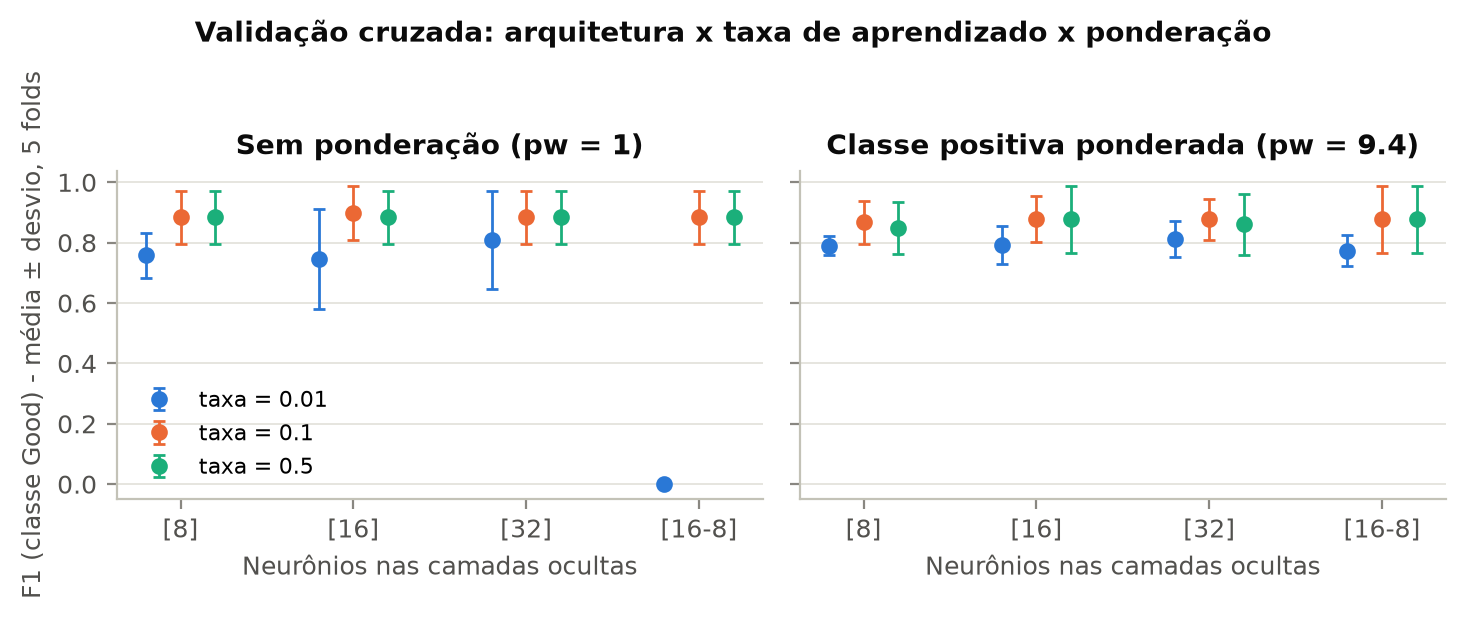
\includegraphics[width=\textwidth]{fig05_grid_cv.png}
\caption{F1 médio de validação (com desvio padrão entre \emph{folds}) para cada arquitetura, taxa de aprendizado e ponderação.}\label{fig:grid}
\end{figure}

Observações:
\begin{itemize}
  \item \textbf{A taxa de aprendizado é o hiperparâmetro mais importante.} Com $\eta = 0{,}01$ a rede não
        converge em 300 épocas: o recall fica entre 0,61 e 0,73 sem ponderação, e a rede 16--8 sequer sai da
        classe majoritária (F1 = 0, acurácia 0,904). Com $\eta = 0{,}1$ ou $0{,}5$ todas as arquiteturas chegam a
        F1 entre 0,85 e 0,90.
  \item \textbf{A arquitetura pouco importa} neste problema: 8, 16, 32 ou 16--8 neurônios dão resultados quase
        idênticos quando $\eta$ é adequado, o que já sugere que a fronteira de decisão é simples.
  \item \textbf{A ponderação da classe positiva troca precisão por recall}: com $w_+ = 9{,}4$ o recall sobe
        (até 1,0 com $\eta = 0{,}01$), mas a precisão cai (0,63 a 0,83) e o F1 fica um pouco menor. Como a
        rede sem ponderação já alcança recall alto (0,94), o balanceamento não compensou.
  \item A melhor configuração foi \textbf{16 neurônios, $\eta = 0{,}1$, $w_+ = 1$}: F1 = 0,899 $\pm$ 0,088,
        acurácia 0,980, recall 0,938, precisão 0,864 e AUC 0,997. Os F1 dos cinco \emph{folds} foram
        0,933, 1,000, 0,857, 0,933 e 0,769: a variação entre \emph{folds} é grande porque cada parte de validação
        tem só 6 ou 7 jogadores \emph{Good}, e um único erro muda o F1 em mais de 0,07.
\end{itemize}

\subsection{Função de ativação}
Com a melhor combinação acima, repetimos a validação cruzada trocando a ativação das camadas ocultas
(Tabela~\ref{tab:ativ}). A sigmoide, proposta no enunciado, foi ligeiramente melhor que tanh e ReLU; as
diferenças (um ou dois jogadores) estão dentro da variação entre \emph{folds}. Haykin (2001) e Adami e Boff
(2026) indicam que funções antissimétricas como a tanh tendem a acelerar o aprendizado; com a taxa de
aprendizado e o número de épocas já ajustados, essa vantagem não apareceu neste problema.

\begin{table}[H]\centering\small
\begin{tabular}{lrrrrrr}
\toprule
Ativação & Acurácia & Precisão & Recall & Especif. & F1 & AUC \\
\midrule
sigmoide & 0,980 & 0,864 & 0,938 & 0,984 & 0,899 $\pm$ 0,088 & 0,997 \\
tanh & 0,977 & 0,861 & 0,910 & 0,984 & 0,883 $\pm$ 0,087 & 0,995 \\
relu & 0,975 & 0,873 & 0,848 & 0,988 & 0,857 $\pm$ 0,113 & 0,993 \\
\bottomrule
\end{tabular}

\caption{Validação cruzada da função de ativação das camadas ocultas (16 neurônios, $\eta = 0{,}1$, $w_+ = 1$, 300 épocas).}\label{tab:ativ}
\end{table}

\subsection{Número de épocas}\label{sec:epocas}
Durante a validação cruzada da configuração escolhida, registramos a cada 10 épocas a perda de treino e a
perda, a acurácia e o F1 de validação (média dos 5 \emph{folds}), Figura~\ref{fig:curvas} e
Tabela~\ref{tab:epocas}. A perda de validação cai rapidamente até cerca de 100 épocas e continua caindo
devagar até 300, sempre acima da perda de treino (a diferença cresce lentamente, um sinal leve de
sobreajuste). O F1 de validação atinge o máximo (0,940) em \textbf{110 épocas} e depois oscila e recua
(0,899 em 300 épocas): as épocas adicionais tornam a rede mais confiante nos casos fáceis sem melhorar os
casos limítrofes. Escolhemos, portanto, 110 épocas para o modelo final.

\begin{figure}[H]\centering
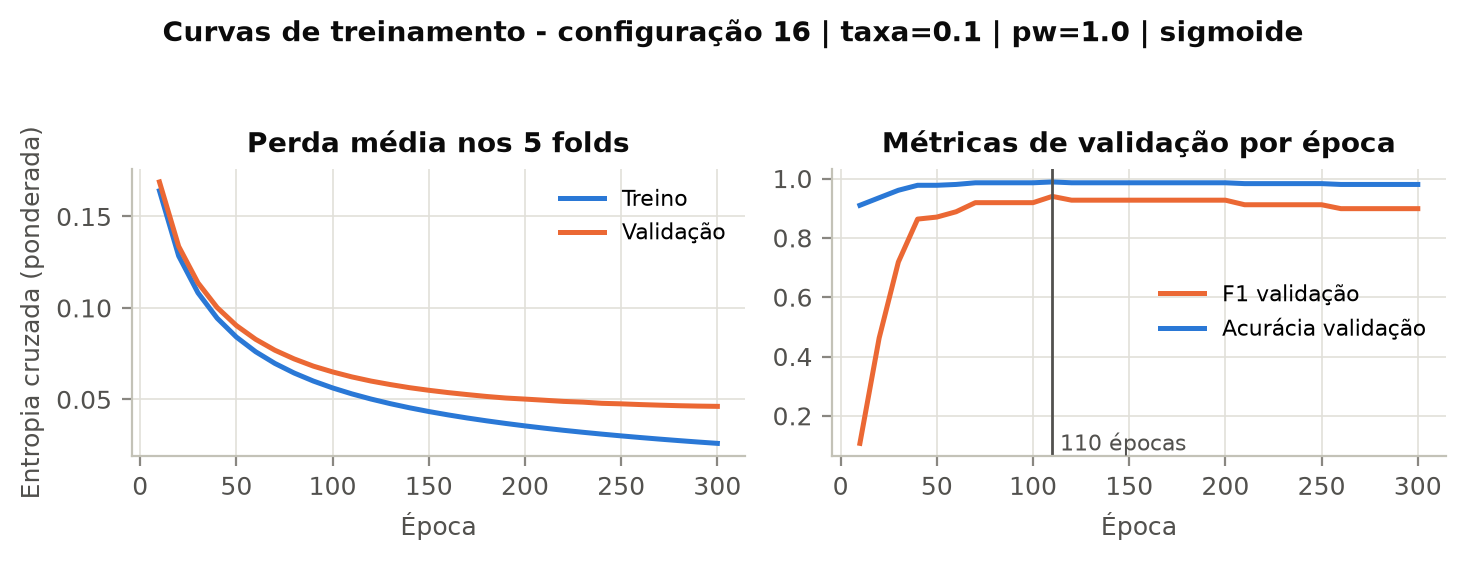
\includegraphics[width=\textwidth]{fig06_curvas_treinamento.png}
\caption{Curvas de treinamento da configuração escolhida (média dos 5 \emph{folds}): perda de treino e validação (esquerda) e acurácia e F1 de validação (direita). A linha vertical marca as 110 épocas escolhidas.}\label{fig:curvas}
\end{figure}

\begin{table}[H]\centering\small
\begin{tabular}{rrrr}
\toprule
Épocas & Perda validação & Acurácia validação & F1 validação \\
\midrule
10 & 0,169 & 0,910 & 0,107 \\
20 & 0,134 & 0,935 & 0,462 \\
30 & 0,114 & 0,961 & 0,719 \\
40 & 0,100 & 0,977 & 0,863 \\
50 & 0,090 & 0,977 & 0,870 \\
60 & 0,083 & 0,980 & 0,888 \\
70 & 0,077 & 0,986 & 0,919 \\
80 & 0,072 & 0,986 & 0,919 \\
90 & 0,068 & 0,986 & 0,919 \\
100 & 0,065 & 0,986 & 0,919 \\
\textbf{110} & 0,062 & 0,989 & \textbf{0,940} \\
120 & 0,060 & 0,986 & 0,927 \\
130 & 0,058 & 0,986 & 0,927 \\
140 & 0,056 & 0,986 & 0,927 \\
150 & 0,055 & 0,986 & 0,927 \\
200 & 0,050 & 0,986 & 0,927 \\
250 & 0,048 & 0,983 & 0,912 \\
300 & 0,046 & 0,980 & 0,899 \\
\bottomrule
\end{tabular}

\caption{Métricas médias de validação em função do número de épocas (configuração 16, $\eta = 0{,}1$, $w_+ = 1$).}\label{tab:epocas}
\end{table}

\subsection{Configuração final e treinamento}
\begin{center}\small
\begin{tabular}{ll}\toprule
Arquitetura & 31 entradas -- 16 neurônios ocultos -- 1 saída (529 parâmetros)\\
Ativações & sigmoide nas camadas oculta e de saída\\
Perda & entropia cruzada binária, $w_+ = 1$\\
Otimização & descida do gradiente em mini-lotes de 32, $\eta = 0{,}1$, sem regularização L2\\
Épocas & 110\\
Inicialização & Glorot uniforme, vieses em zero, 5 sementes diferentes (0 a 4)\\
\bottomrule\end{tabular}
\end{center}
Com essa configuração a rede foi treinada em todo o conjunto de treino (355 jogadores). Cada treinamento
leva cerca de 3 s em Python puro. A perda de treino cai de 0,13--0,17 (época 10) para 0,04--0,05 (época 110),
conforme a semente.

% =============================================================================
\section{Avaliação e ajuste}\label{sec:avaliacao}

\subsection{Métricas}
As métricas seguem as definições apresentadas na disciplina e em Faceli et al. (2021).
Todas foram implementadas em \texttt{src/metricas.py} a partir da matriz de confusão, com a
classe \emph{Good} como positiva (VP = verdadeiros positivos, FP = falsos positivos, VN = verdadeiros
negativos, FN = falsos negativos):
\[
\begin{aligned}
\text{Acurácia} &= \frac{VP+VN}{VP+FP+VN+FN}, & \text{Erro} &= 1 - \text{Acurácia},\\[4pt]
\text{Precisão} &= \frac{VP}{VP+FP}, & \text{Recall (sensibilidade)} &= \frac{VP}{VP+FN},\\[4pt]
\text{Especificidade} &= \frac{VN}{VN+FP}, & \text{F1} &= \frac{2\cdot\text{Precisão}\cdot\text{Recall}}{\text{Precisão}+\text{Recall}}.
\end{aligned}
\]
A \textbf{curva ROC} é construída ordenando as instâncias pela probabilidade prevista e percorrendo todos os
limiares possíveis, calculando em cada um a taxa de verdadeiros positivos (TPR = recall) e a de falsos
positivos (FPR = $1-$especificidade); a \textbf{AUC} é a área sob a curva, calculada pela regra do trapézio
(FAWCETT, 2006).

\subsection{Resultados no conjunto de teste}\label{sec:execucoes}
A configuração final foi executada \textbf{cinco vezes} com sementes de inicialização diferentes, sempre
treinando nos 355 jogadores de treino e avaliando nos 153 de teste (Tabela~\ref{tab:exec}). Os resultados
são estáveis: acurácia 0,974 $\pm$ 0,005, erro 0,026, precisão 0,818 $\pm$ 0,038, recall 0,947 $\pm$ 0,030,
especificidade 0,977 $\pm$ 0,006, F1 0,877 $\pm$ 0,020 e AUC 0,995 $\pm$ 0,001. Em todas as execuções
a rede encontra 14 ou 15 dos 15 jogadores \emph{Good} e comete entre 2 e 4 falsos positivos.

\begin{table}[H]\centering
\resizebox{\textwidth}{!}{\begin{tabular}{lrrrrrrrrrrr}
\toprule
Execução & VP & FP & VN & FN & Acurácia & Erro & Precisão & Recall & Especif. & F1 & AUC \\
\midrule
semente 0 & 15 & 4 & 134 & 0 & 0,974 & 0,026 & 0,789 & 1,000 & 0,971 & 0,882 & 0,995 \\
semente 1 (mediana) & 14 & 3 & 135 & 1 & 0,974 & 0,026 & 0,824 & 0,933 & 0,978 & 0,875 & 0,995 \\
semente 2 & 14 & 3 & 135 & 1 & 0,974 & 0,026 & 0,824 & 0,933 & 0,978 & 0,875 & 0,994 \\
semente 3 & 14 & 2 & 136 & 1 & 0,980 & 0,020 & 0,875 & 0,933 & 0,986 & 0,903 & 0,996 \\
semente 4 & 14 & 4 & 134 & 1 & 0,967 & 0,033 & 0,778 & 0,933 & 0,971 & 0,848 & 0,994 \\
\midrule
\textbf{Média $\pm$ desvio} & & & & & 0,974 $\pm$ 0,005 & 0,026 $\pm$ 0,005 & 0,818 $\pm$ 0,038 & 0,947 $\pm$ 0,030 & 0,977 $\pm$ 0,006 & 0,877 $\pm$ 0,020 & 0,995 $\pm$ 0,001 \\
\bottomrule
\end{tabular}
}
\caption{Cinco execuções da configuração final no conjunto de teste (153 jogadores, 15 \emph{Good}).}\label{tab:exec}
\end{table}

A Figura~\ref{fig:mc} mostra a matriz de confusão da execução mediana (semente 1) e a Figura~\ref{fig:roc}
sua curva ROC. A AUC de 0,995 indica que a rede ordena quase perfeitamente os jogadores: existe um limiar
que separa todos os \emph{Good} com apenas 3 falsos positivos, e o limiar padrão de 0,5 fica muito perto do
canto superior esquerdo.

\begin{figure}[H]\centering
\begin{minipage}{0.46\textwidth}\centering
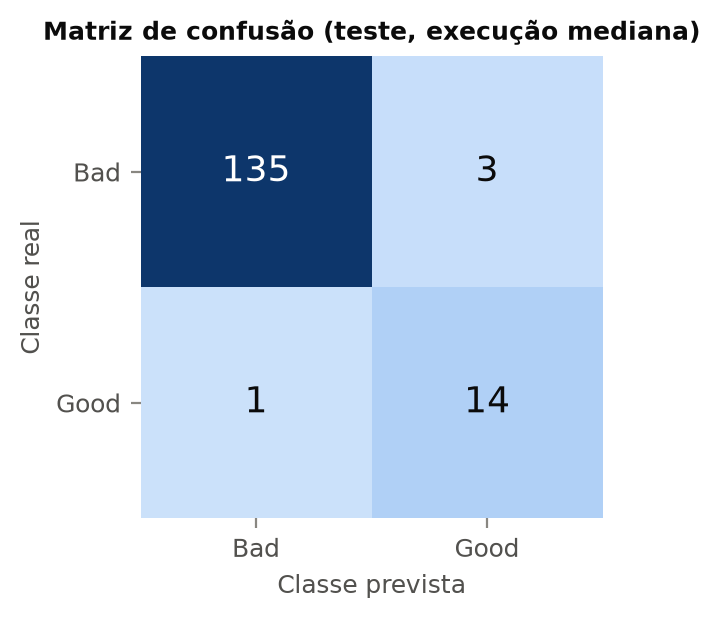
\includegraphics[width=\textwidth]{fig07_matriz_confusao.png}
\caption{Matriz de confusão da execução mediana no teste.}\label{fig:mc}
\end{minipage}\hfill
\begin{minipage}{0.5\textwidth}\centering
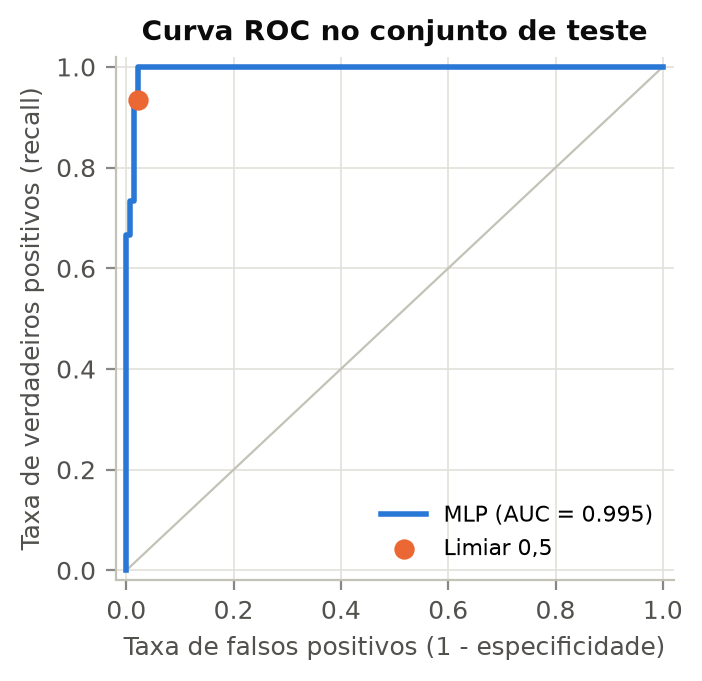
\includegraphics[width=\textwidth]{fig08_roc.png}
\caption{Curva ROC da execução mediana no teste; o ponto marca o limiar 0,5.}\label{fig:roc}
\end{minipage}
\end{figure}

\subsection{Análise dos erros}
A Tabela~\ref{tab:erros} lista os quatro jogadores classificados incorretamente pela execução mediana.
Todos estão na faixa de 19,5 a 21,4 pontos por jogo, exatamente na fronteira entre as classes vista na
Figura~\ref{fig:pts}, e as probabilidades previstas ficam perto de 0,5. Terry Rozier é o único jogador do
dataset com mais de 20 pontos rotulado \emph{Bad}; Dejounte Murray (20,9 PTS, \emph{Good}) recebeu 0,478 e
ficou logo abaixo do limiar. Cade Cunningham, com 19,9 PTS em apenas 12 jogos, e Tyrese Maxey (19,5 PTS)
foram previstos \emph{Good} por terem perfil estatístico de titular com alto volume de arremessos. Ou seja, a
rede erra apenas onde o próprio rótulo é ambíguo.

\begin{table}[H]\centering\small
\begin{tabular}{lrrrrll}
\toprule
Jogador & G & MP & PTS & Prob. Good & Real & Previsto \\
\midrule
Terry Rozier & 52 & 35,6 & 21,4 & 0,672 & Bad & Good \\
Dejounte Murray & 56 & 36,4 & 20,9 & 0,478 & Good & Bad \\
Cade Cunningham & 12 & 33,3 & 19,9 & 0,707 & Bad & Good \\
Tyrese Maxey & 41 & 32,5 & 19,5 & 0,522 & Bad & Good \\
\bottomrule
\end{tabular}

\caption{Jogadores classificados incorretamente pela execução mediana (G = jogos, MP = minutos por jogo).}\label{tab:erros}
\end{table}

\subsection{Comparação com modelos de referência}\label{sec:baselines}
Para julgar se os números são bons, comparamos com dois modelos de referência avaliados no mesmo teste
(Tabela~\ref{tab:comp}, Figura~\ref{fig:comp}):
\begin{itemize}
  \item \textbf{Classe majoritária}: prever sempre \emph{Bad}. Acurácia de 0,902, mas recall, precisão e F1 iguais
        a zero. Mostra por que a acurácia sozinha engana neste dataset.
  \item \textbf{Regra ``PTS $\ge$ limiar''}: o limiar (20,2 pontos) foi escolhido no conjunto de treino maximizando
        o F1, onde separa perfeitamente as classes. No teste acerta 152 dos 153 jogadores (F1 = 0,968); o único
        erro é Terry Rozier.
\end{itemize}

\begin{table}[H]\centering\footnotesize
\begin{tabular}{lrrrrrr}
\toprule
Modelo & Acurácia & Precisão & Recall & Especif. & F1 & AUC \\
\midrule
Classe majoritária (sempre Bad) & 0,902 & 0,000 & 0,000 & 1,000 & 0,000 & 0,500 \\
Regra PTS $\geq$ 20,2 & 0,993 & 0,938 & 1,000 & 0,993 & 0,968 & 0,998 \\
MLP sem atributos de pontuação (média de 5) & 0,957 & 0,750 & 0,840 & 0,970 & 0,792 & 0,981 \\
MLP completa (média de 5) & 0,974 & 0,818 & 0,947 & 0,977 & 0,877 & 0,995 \\
\bottomrule
\end{tabular}

\caption{Comparação no conjunto de teste entre os modelos de referência e a MLP nos dois cenários.}\label{tab:comp}
\end{table}

\begin{figure}[H]\centering
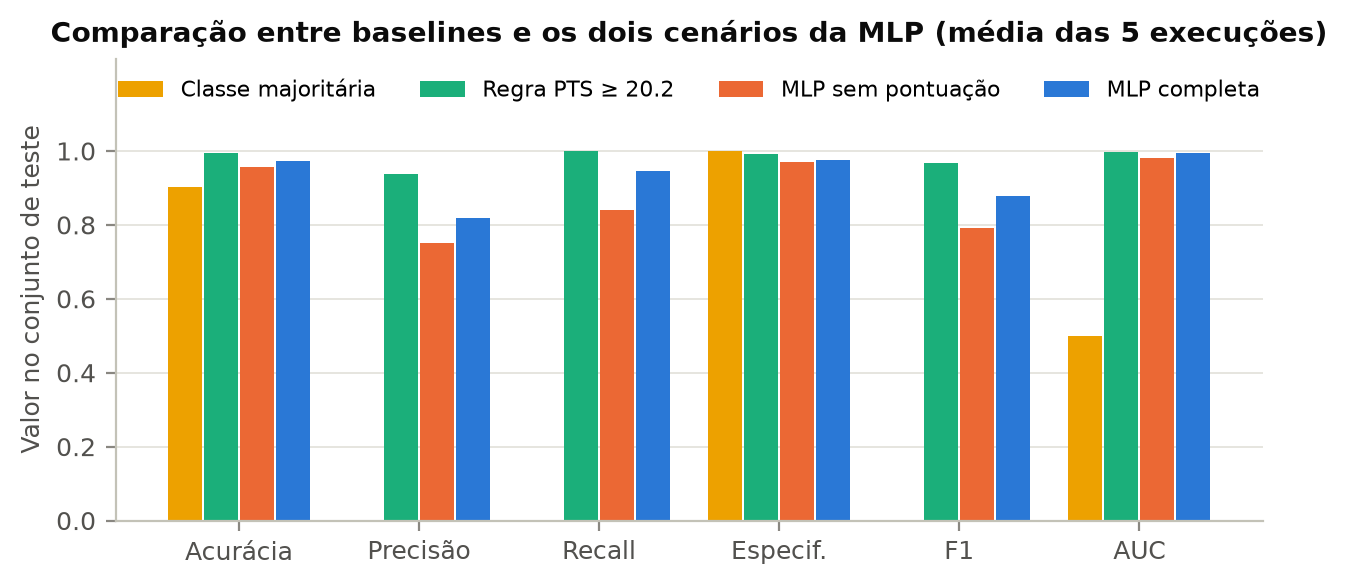
\includegraphics[width=\textwidth]{fig10_comparacao.png}
\caption{Métricas no conjunto de teste para os modelos de referência e os dois cenários da MLP.}\label{fig:comp}
\end{figure}

A MLP supera com folga a classe majoritária em todas as métricas que envolvem a classe \emph{Good}, mas fica
\emph{abaixo} da regra de um único atributo. Isso não é um defeito da implementação, e sim uma consequência do
problema: o rótulo é praticamente uma função de limiar de PTS, e a regra incorpora esse conhecimento
diretamente, enquanto a rede precisa descobri-lo a partir de 31 atributos correlacionados com apenas 34
exemplos positivos. A rede distribui a decisão entre PTS e seus componentes (FG, FT, 2P, FGA\ldots), o que a
torna um pouco ``borrada'' justamente na fronteira (Seção~\ref{sec:importancia}).

\subsection{Resumo dos ajustes realizados}
O ajuste de hiperparâmetros teve impacto concreto:
\begin{itemize}
  \item \textbf{Taxa de aprendizado}: de 0,01 para 0,1 elevou o F1 de validação de 0,745 para 0,899 na rede de
        16 neurônios e resgatou a rede 16--8 do colapso na classe majoritária.
  \item \textbf{Épocas}: de 300 para 110 elevou o F1 de validação de 0,899 para 0,940 e reduziu o tempo de
        treino em 63\%.
  \item \textbf{Ponderação da classe positiva}: aumentou o recall, mas reduziu a precisão e o F1; não foi adotada.
  \item \textbf{Arquitetura e ativação}: efeito pequeno; mantivemos a opção mais simples (16 neurônios, sigmoide).
\end{itemize}

% =============================================================================
\section{Interpretação e conclusão}\label{sec:interpretacao}

\subsection{Eficácia do modelo}
A MLP implementada do zero resolve o problema com acurácia de 97,4\% e AUC de 0,995, encontrando em média
94,7\% dos jogadores \emph{Good} e errando quase só em jogadores com 19 a 21 pontos por jogo. Os resultados
são consistentes entre a validação cruzada (F1 0,94 em 110 épocas) e o teste (F1 0,88), e estáveis entre
sementes (desvio de 0,02 no F1), o que indica que o treinamento está funcionando e que não há sobreajuste
grave. Por outro lado, a comparação com a regra ``PTS $\ge$ 20,2'' mostra que a tarefa, da forma como o rótulo
foi definido, é essencialmente unidimensional: um classificador não linear com 529 parâmetros não traz
ganho sobre um limiar em uma variável. O valor da MLP aqui está em ter aprendido essa estrutura
\emph{sem que ninguém a informasse}.

\subsection{Variáveis com maior impacto}\label{sec:importancia}
Três evidências, todas calculadas manualmente, apontam para as mesmas variáveis:

\begin{enumerate}
  \item \textbf{Correlação com o alvo} (Figura~\ref{fig:corr}): FT, PTS, FTA, FG, FGA, 2PA e 2P têm $r > 0{,}67$.
  \item \textbf{Importância por permutação} (BREIMAN, 2001) (Figura~\ref{fig:imp}, Tabela~\ref{tab:impA}): para cada atributo,
        embaralhamos seus valores no conjunto de teste (destruindo sua relação com o alvo, mas preservando a
        distribuição) e medimos a queda de AUC e de F1 do modelo final, média de 20 permutações. PTS é o
        atributo mais importante (queda de F1 de 0,119), seguido de 2P (0,092), 2PA (0,076), FT (0,074) e FG
        (0,073). As quedas de AUC são pequenas (no máximo 0,003) porque esses atributos são
        \emph{redundantes}: PTS $= 2\cdot$2P $+ 3\cdot$3P $+$ FT, de modo que, ao embaralhar um deles, a rede
        recupera quase toda a informação pelos outros. Atributos de eficiência (FG\%, 2P\%, eFG\%), de rebote e
        de defesa (BLK, ORB) têm importância próxima de zero.
  \item \textbf{Pesos de conexão} (generalização do método de Garson (1991): produto das matrizes de pesos em valor
        absoluto): com 31 entradas correlacionadas, os pesos ficam distribuídos de forma quase uniforme
        (0,027 a 0,043 por atributo), com PTS, FG e FTA entre os maiores. Esse método é menos informativo que a
        permutação neste caso, pois mede a estrutura da rede e não o efeito sobre a previsão.
\end{enumerate}

\begin{figure}[H]\centering
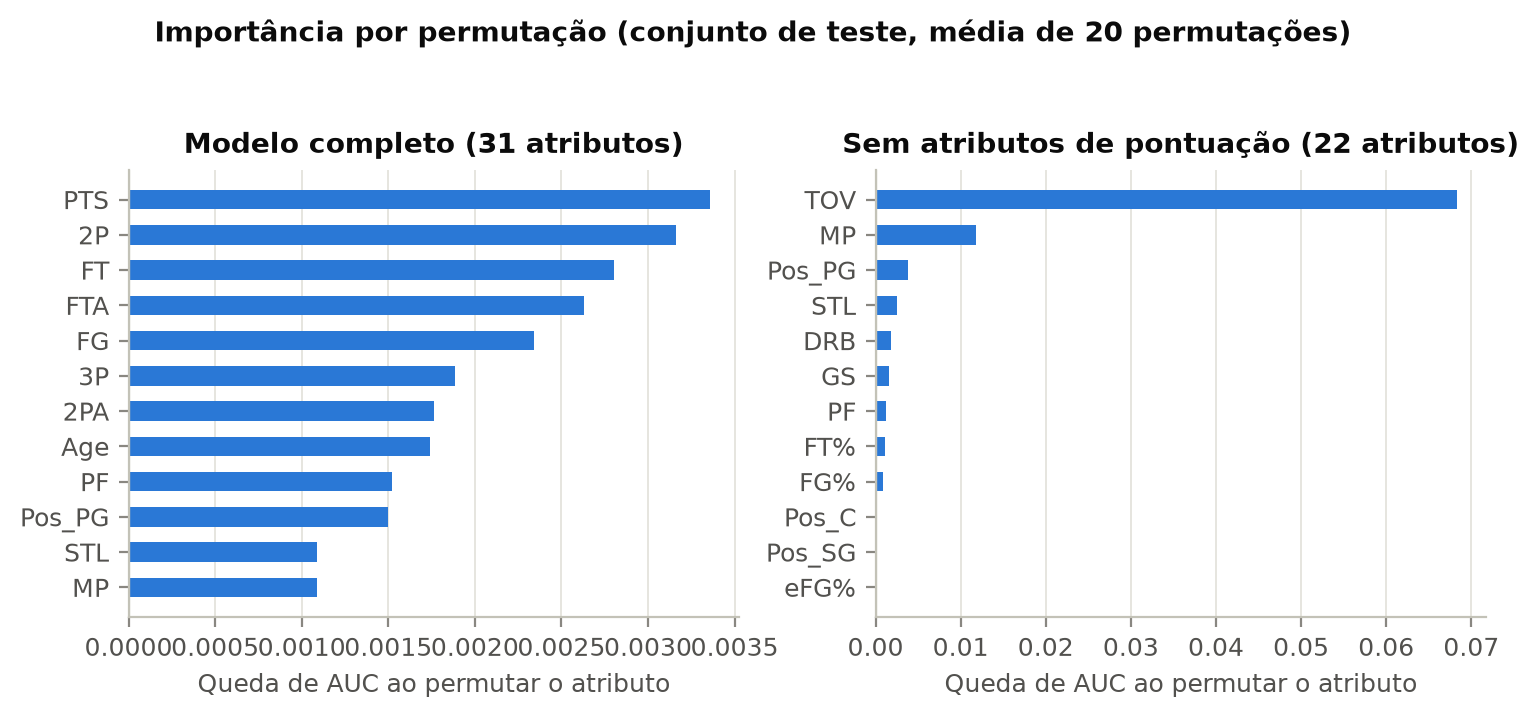
\includegraphics[width=\textwidth]{fig09_importancia.png}
\caption{Importância por permutação (queda de AUC no teste) dos 12 atributos mais importantes no modelo completo (esquerda) e no cenário sem atributos de pontuação (direita). Note a escala diferente dos dois painéis.}\label{fig:imp}
\end{figure}

\begin{table}[H]\centering\footnotesize
\begin{minipage}[t]{0.48\textwidth}\centering
\resizebox{\textwidth}{!}{\begin{tabular}{lrrr}
\toprule
Atributo & Queda AUC & Queda F1 & Peso conexão \\
\midrule
PTS & 0,003 & 0,119 & 0,043 \\
2P & 0,003 & 0,092 & 0,038 \\
FT & 0,003 & 0,074 & 0,038 \\
FTA & 0,003 & 0,055 & 0,039 \\
FG & 0,002 & 0,073 & 0,042 \\
3P & 0,002 & 0,046 & 0,037 \\
2PA & 0,002 & 0,076 & 0,034 \\
Age & 0,002 & 0,005 & 0,038 \\
PF & 0,002 & 0,013 & 0,036 \\
Pos\_PG & 0,001 & 0,021 & 0,039 \\
\bottomrule
\end{tabular}
}
\caption{Modelo completo: dez atributos mais importantes.}\label{tab:impA}
\end{minipage}\hfill
\begin{minipage}[t]{0.48\textwidth}\centering
\resizebox{\textwidth}{!}{\begin{tabular}{lrrr}
\toprule
Atributo & Queda AUC & Queda F1 & Peso conexão \\
\midrule
TOV & 0,068 & 0,579 & 0,106 \\
MP & 0,012 & 0,282 & 0,084 \\
Pos\_PG & 0,004 & 0,011 & 0,051 \\
STL & 0,003 & 0,006 & 0,041 \\
DRB & 0,002 & 0,078 & 0,032 \\
GS & 0,002 & 0,098 & 0,045 \\
PF & 0,001 & -0,003 & 0,049 \\
FT\% & 0,001 & 0,051 & 0,049 \\
FG\% & 0,001 & 0,004 & 0,051 \\
Pos\_C & 0,000 & -0,007 & 0,034 \\
\bottomrule
\end{tabular}
}
\caption{Cenário sem pontuação: dez atributos mais importantes.}\label{tab:impB}
\end{minipage}
\end{table}

\subsection{Cenário sem atributos de pontuação}
Como o rótulo é quase determinado por PTS, fizemos uma pergunta mais interessante: \emph{é possível identificar
um jogador \emph{Good} sem olhar para a pontuação?} Treinamos a mesma configuração removendo os nove atributos de
volume de pontuação (PTS, FG, FGA, 3P, 3PA, 2P, 2PA, FT, FTA), ficando com 22 atributos: idade, uso (G, GS, MP),
percentuais de aproveitamento, rebotes, assistências, roubos, tocos, erros de posse, faltas e posição.
Os resultados das cinco execuções estão na Tabela~\ref{tab:execB} e a matriz de confusão mediana na
Figura~\ref{fig:mcB}. A rede ainda alcança AUC de 0,981, acurácia de 0,957 e recall de 0,84, mas a precisão cai
para 0,75 (F1 0,79): o problema fica genuinamente mais difícil.

\begin{table}[H]\centering
\resizebox{\textwidth}{!}{\begin{tabular}{lrrrrrrrrrrr}
\toprule
Execução & VP & FP & VN & FN & Acurácia & Erro & Precisão & Recall & Especif. & F1 & AUC \\
\midrule
semente 0 & 13 & 4 & 134 & 2 & 0,961 & 0,039 & 0,765 & 0,867 & 0,971 & 0,812 & 0,984 \\
semente 1 & 12 & 4 & 134 & 3 & 0,954 & 0,046 & 0,750 & 0,800 & 0,971 & 0,774 & 0,981 \\
semente 2 & 13 & 4 & 134 & 2 & 0,961 & 0,039 & 0,765 & 0,867 & 0,971 & 0,812 & 0,981 \\
semente 3 & 12 & 4 & 134 & 3 & 0,954 & 0,046 & 0,750 & 0,800 & 0,971 & 0,774 & 0,974 \\
semente 4 (mediana) & 13 & 5 & 133 & 2 & 0,954 & 0,046 & 0,722 & 0,867 & 0,964 & 0,788 & 0,984 \\
\midrule
\textbf{Média $\pm$ desvio} & & & & & 0,957 $\pm$ 0,004 & 0,043 $\pm$ 0,004 & 0,750 $\pm$ 0,017 & 0,840 $\pm$ 0,037 & 0,970 $\pm$ 0,003 & 0,792 $\pm$ 0,019 & 0,981 $\pm$ 0,004 \\
\bottomrule
\end{tabular}
}
\caption{Cinco execuções da MLP sem os atributos de pontuação, no conjunto de teste.}\label{tab:execB}
\end{table}

\begin{figure}[H]\centering
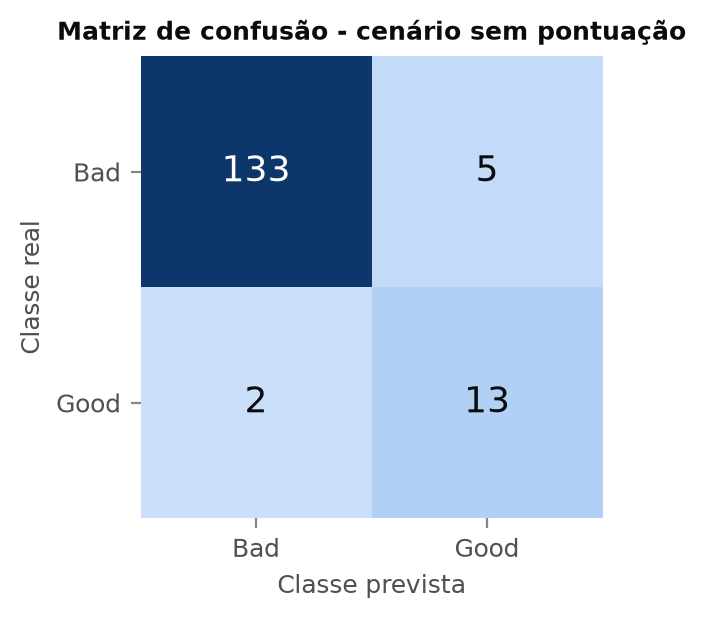
\includegraphics[width=0.42\textwidth]{fig07b_matriz_confusao_sem_pontuacao.png}
\caption{Matriz de confusão da execução mediana no cenário sem atributos de pontuação.}\label{fig:mcB}
\end{figure}

Neste cenário a importância por permutação (Figura~\ref{fig:imp}, direita; Tabela~\ref{tab:impB}) é muito
mais concentrada: \textbf{erros de posse (TOV)} dominam (queda de AUC de 0,068 e de F1 de 0,58), seguidos de
\textbf{minutos por jogo (MP)} (0,012 e 0,28), posição de armador (Pos\_PG), roubos (STL), rebotes defensivos
(DRB) e jogos como titular (GS). A interpretação é consistente com o basquete: os grandes pontuadores são
jogadores de alto \emph{uso}, que ficam com a bola nas mãos por mais tempo (e por isso cometem mais erros de
posse) e jogam mais minutos. Os erros desse modelo são informativos: ele classifica como \emph{Bad} Jimmy Butler e
Kawhi Leonard, astros eficientes que pontuam muito com poucos erros de posse, e como \emph{Good} armadores de alto
uso com menos de 20 pontos, como Tyrese Haliburton, Jrue Holiday e Kevin Porter Jr.

\subsection{Limitações}
\begin{itemize}
  \item \textbf{Poucos exemplos positivos}: 34 jogadores \emph{Good} no treino e 15 no teste. Cada erro no teste muda
        a precisão ou o recall em cerca de 0,06, por isso reportamos média e desvio de cinco execuções e usamos
        validação cruzada em vez de um único conjunto de validação.
  \item \textbf{Rótulo quase determinístico}: a definição de \emph{Good} como ``20 ou mais pontos'' torna o problema
        fácil para um limiar e deixa pouco espaço para a rede mostrar vantagem.
  \item \textbf{Linhas por time}: optamos por manter apenas o total (TOT) de jogadores trocados; outra escolha
        (manter cada passagem) mudaria ligeiramente o conjunto.
  \item \textbf{Custo computacional}: Python puro é lento (16 s por treinamento de 300 épocas); o grid foi viável
        porque o dataset é pequeno.
\end{itemize}

\subsection{Sugestões de melhoria}
\begin{enumerate}
  \item \textbf{Ajustar o limiar de decisão} pela curva ROC ou pela curva precisão-recall na validação
        (em vez de fixar 0,5); a AUC de 0,995 mostra que há limiares com menos falsos positivos.
  \item \textbf{Seleção de atributos}: remover atributos redundantes (manter PTS e descartar FG, 2P, FT\ldots, ou o
        contrário) reduziria a ``diluição'' da decisão na fronteira e aproximaria a rede da regra de limiar.
  \item \textbf{Parada antecipada} (\emph{early stopping}) com base na perda de validação, em vez de fixar as épocas,
        e \textbf{regularização L2} (já implementada, com $\lambda = 0$ nos experimentos) ou \emph{dropout}
        (GOODFELLOW; BENGIO; COURVILLE, 2016).
  \item \textbf{Otimizadores com momento} (momentum, Adam) para acelerar a convergência e reduzir a sensibilidade
        à taxa de aprendizado, que foi o hiperparâmetro mais crítico (KINGMA; BA, 2015). O material complementar
        da disciplina discute critérios práticos para essa escolha (DATA SCIENCE ACADEMY, [20-{}-]).
  \item \textbf{Validação cruzada repetida} ou \emph{bootstrap} (ADAMI, 2026; KOHAVI, 1995) para intervalos de confiança das métricas,
        dado o pequeno número de positivos.
  \item \textbf{Um rótulo mais rico}: usar uma medida composta de desempenho (por exemplo, pontos, rebotes,
        assistências e eficiência combinados) tornaria o problema mais interessante e aproveitaria melhor a
        capacidade não linear da MLP, como sugere o cenário sem pontuação.
\end{enumerate}

\subsection{Conclusão}
Implementamos do zero uma MLP completa (arquitetura configurável, inicialização Glorot/He, ativações
sigmoide/tanh/ReLU, entropia cruzada ponderada, retropropagação verificada numericamente e descida do
gradiente em mini-lotes) e um conjunto de métricas manuais (matriz de confusão, acurácia, erro, precisão,
recall, especificidade, F1 e curva ROC/AUC). Com um protocolo rigoroso (limpeza com remoção de duplicatas,
padronização só com estatísticas do treino, validação cruzada estratificada para os hiperparâmetros e teste
usado uma única vez), a rede final atinge acurácia de 97,4\% e AUC de 0,995. As principais aprendizagens
foram: (i) a taxa de aprendizado e o número de épocas importam mais que a arquitetura; (ii) com classes
desbalanceadas, acurácia é insuficiente e é preciso olhar recall, precisão, F1 e ROC; (iii) entender os dados
(aqui, que o rótulo é um limiar de PTS) é tão importante quanto o modelo, pois uma regra trivial empata ou
supera a rede; e (iv) sem os atributos de pontuação a rede ainda identifica bons pontuadores pelo seu
perfil de uso (TOV, MP), o que é um resultado não óbvio e sugere trabalhos futuros com rótulos mais
elaborados.

% =============================================================================
\section*{Referências}
\addcontentsline{toc}{section}{Referências}
\begingroup
\small
\setlength{\parindent}{0pt}
\setlength{\parskip}{8pt}
\raggedright

ADAMI, André Gustavo. \textbf{Métodos de avaliação de desempenho}. Caxias do Sul: Universidade de Caxias do
Sul, 2026. Slides de aula (Aula 7) da disciplina FBX4054 -- Inteligência Computacional, Profa. Elisa Boff.
Disponível no ambiente virtual de aprendizagem da disciplina. Acesso em: 3 nov. 2026.

ADAMI, André Gustavo; BOFF, Elisa. \textbf{Redes neurais artificiais}. Caxias do Sul: Universidade de Caxias
do Sul, 2026. Slides de aula (Aula 9) da disciplina FBX4054 -- Inteligência Computacional. Disponível no
ambiente virtual de aprendizagem da disciplina. Acesso em: 3 nov. 2026.

BOFF, Elisa. \textbf{Trabalho de implementação de rede neural MLP}: previsão de desempenho de jogadores de
basquete. Caxias do Sul: Universidade de Caxias do Sul, 2026. Enunciado da Atividade Avaliativa 2 e dataset
da disciplina FBX4054 -- Inteligência Computacional. Disponível no ambiente virtual de aprendizagem da
disciplina. Acesso em: 3 nov. 2026.

BREIMAN, Leo. Random forests. \textbf{Machine Learning}, v. 45, n. 1, p. 5--32, 2001.

DATA SCIENCE ACADEMY. Como escolher os hiperparâmetros de uma rede neural. In: DATA SCIENCE ACADEMY.
\textbf{Deep Learning Book}. [\emph{S. l.}], [20-{}-]. Disponível em:
\url{https://www.deeplearningbook.com.br/como-escolher-os-hiperparametros-de-uma-rede-neural/}.
Acesso em: 3 nov. 2026.

FACELI, Katti \emph{et al.} \textbf{Inteligência artificial}: uma abordagem de aprendizado de máquina. 2. ed.
Rio de Janeiro: LTC, 2021. E-book. ISBN 9788521637509.

FAWCETT, Tom. An introduction to ROC analysis. \textbf{Pattern Recognition Letters}, v. 27, n. 8,
p. 861--874, 2006.

GARSON, G. David. Interpreting neural-network connection weights. \textbf{AI Expert}, v. 6, n. 4,
p. 46--51, 1991.

GLOROT, Xavier; BENGIO, Yoshua. Understanding the difficulty of training deep feedforward neural networks.
In: INTERNATIONAL CONFERENCE ON ARTIFICIAL INTELLIGENCE AND STATISTICS, 13., 2010, Sardinia.
\textbf{Proceedings} [...]. [\emph{S. l.}]: PMLR, 2010. v. 9, p. 249--256.

GOODFELLOW, Ian; BENGIO, Yoshua; COURVILLE, Aaron. \textbf{Deep learning}. Cambridge: MIT Press, 2016.

HAYKIN, Simon. \textbf{Redes neurais}: princípios e prática. 2. ed. Porto Alegre: Bookman, 2001.

HE, Kaiming \emph{et al.} Delving deep into rectifiers: surpassing human-level performance on ImageNet
classification. In: IEEE INTERNATIONAL CONFERENCE ON COMPUTER VISION, 2015, Santiago.
\textbf{Proceedings} [...]. [\emph{S. l.}]: IEEE, 2015. p. 1026--1034.

HUNTER, John D. Matplotlib: a 2D graphics environment. \textbf{Computing in Science \& Engineering}, v. 9,
n. 3, p. 90--95, 2007.

KINGMA, Diederik P.; BA, Jimmy. Adam: a method for stochastic optimization. In: INTERNATIONAL CONFERENCE ON
LEARNING REPRESENTATIONS, 3., 2015, San Diego. \textbf{Proceedings} [...]. [\emph{S. l.}: \emph{s. n.}], 2015.
Disponível em: \url{https://arxiv.org/abs/1412.6980}. Acesso em: 3 nov. 2026.

KOHAVI, Ron. A study of cross-validation and bootstrap for accuracy estimation and model selection. In:
INTERNATIONAL JOINT CONFERENCE ON ARTIFICIAL INTELLIGENCE, 14., 1995, Montreal. \textbf{Proceedings} [...].
San Francisco: Morgan Kaufmann, 1995. v. 2, p. 1137--1143.

LUGER, George F. \textbf{Inteligência artificial}. 6. ed. São Paulo: Pearson, 2013. E-book.
ISBN 9788581435503.

MCKINNEY, Wes. Data structures for statistical computing in Python. In: PYTHON IN SCIENCE CONFERENCE, 9.,
2010, Austin. \textbf{Proceedings} [...]. [\emph{S. l.}: \emph{s. n.}], 2010. p. 56--61.

ROSENBLATT, Frank. The perceptron: a probabilistic model for information storage and organization in the
brain. \textbf{Psychological Review}, v. 65, n. 6, p. 386--408, 1958.

RUMELHART, David E.; HINTON, Geoffrey E.; WILLIAMS, Ronald J. Learning representations by
back-propagating errors. \textbf{Nature}, v. 323, p. 533--536, 1986.

RUSSELL, Stuart J.; NORVIG, Peter. \textbf{Inteligência artificial}: uma abordagem moderna. 4. ed.
Rio de Janeiro: GEN LTC, 2022. E-book. ISBN 9788595159495.

SILVA, Fabrício M. \emph{et al.} \textbf{Inteligência artificial}. Porto Alegre: SAGAH, 2018. E-book.
Disponível em: Minha Biblioteca.
\endgroup

\appendix
\section{Código-fonte e reprodução}\label{apx:codigo}
\begin{center}\footnotesize
\begin{tabular}{lp{10.2cm}}\toprule
Arquivo & Conteúdo\\\midrule
\texttt{src/preparacao\_dados.py} & carga, limpeza, codificação, divisão estratificada e padronização (pandas)\\
\texttt{src/mlp.py} & classe \texttt{MLP}: camadas, inicialização, ativações, perda, retropropagação, treino\\
\texttt{src/metricas.py} & matriz de confusão, acurácia, erro, precisão, recall, especificidade, F1, ROC/AUC\\
\texttt{src/experimentos.py} & validação cruzada, grid, ativações, épocas, execuções finais, baselines, cenário B\\
\texttt{src/importancia.py} & importância por permutação e por pesos de conexão\\
\texttt{src/visualizacoes.py} & figuras (matplotlib)\\
\texttt{src/gerar\_tabelas.py} & tabelas LaTeX deste relatório a partir dos resultados\\
\texttt{tests/test\_mlp.py} & testes: gradiente numérico, XOR, exportação, métricas\\
\texttt{dados/} & CSV original e dados processados (treino/teste padronizados)\\
\texttt{resultados/} & \texttt{experimentos.json}, modelos treinados, importâncias\\
\bottomrule\end{tabular}
\end{center}

Para reproduzir todos os resultados (Python 3.14, pacotes \texttt{pandas} e \texttt{matplotlib}):
\begin{lstlisting}
python -m unittest discover -s tests      # testes de corretude
python src/preparacao_dados.py            # etapa 1
python src/experimentos.py                # etapas 3 e 4 (cerca de 4 min em 8 processos)
python src/importancia.py                 # etapa 5
python src/visualizacoes.py               # figuras
python src/gerar_tabelas.py               # tabelas do relatório
cd relatorio && tectonic relatorio.tex    # este PDF
\end{lstlisting}
Todas as sementes aleatórias estão fixadas; os números deste relatório são reproduzidos exatamente.

\end{document}
